\documentclass[a4paper]{article}

\usepackage{html}
\usepackage{hthtml}
\usepackage{xspace}
\usepackage{url}
\usepackage{graphicx}

\newcommand{\Jason}[0]{\htlink{\textit{\textbf{Jason}}}{http://jason.sf.net}\xspace}

\begin{document}

\html{
\begin{rawhtml}
  <div class=title>Getting started with <b><i>Jason</i></b></div>
  <br/><br/>
\end{rawhtml}
}


% -----------------------------------------------------------------

This document aims to help you install and run \Jason, as well as
developing a simple multi-agent system using \Jason.

\tableofcontents


\section{Installation and Configuration}

\begin{enumerate}
\item Java JDK >= 5.0 is required (\url{http://java.sun.com});
\item Download \Jason from \url{http://jason.sf.net};
\item Create a folder for your \Jason installation and decompress the
  distribution file in it;
\item You can now execute \Jason:
  \begin{itemize}
  \item Windows: Double-click on Jason.exe
  \item MacOS: Double-click on Jason.app
  \item Linux: run bin/jason.sh
  \end{itemize}

  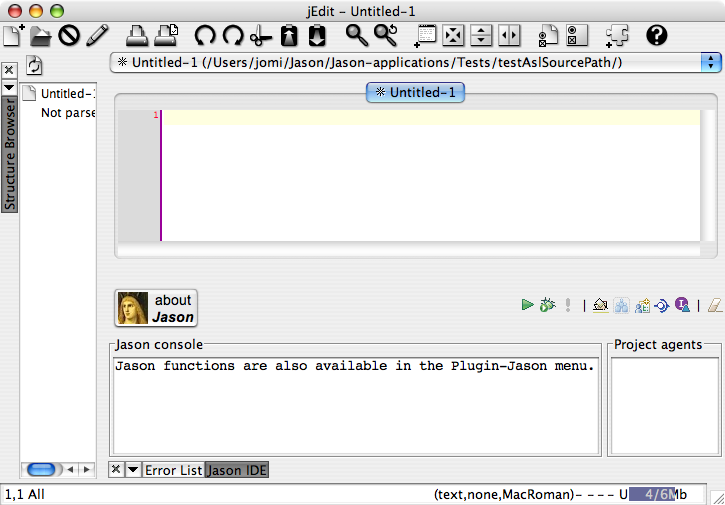
\includegraphics{figures/screen-initial.png}

  As you can see, \Jason runs as a plugin of
  \htlink{jEdit}{http://www.jedit.org/} (a text editor developed in
  Java). This is useful because, although in \Jason agents are
  programmed in a variant of AgentSpeak, in most cases you'll need to
  do some Java programming (e.g., if you want to create an environment
  where the agents are situated).

\item In some cases, it might be necessary to configure the directory
  where Java JDK is installed. This can be done in the menu
  Plugins -> Plugins Options -> Jason:

  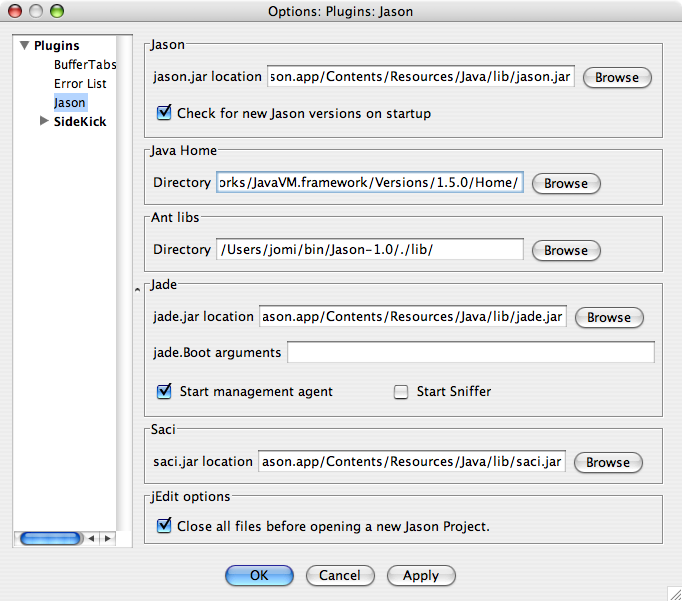
\includegraphics{figures/screen-conf.png}

\item Done! It's that simple!
\end{enumerate}

You are now ready to run a \Jason multi-agent system, as we explain
next.

\section{Execution of an example}

\Jason comes with many examples and demos. The examples are
multi-agent system applications for simple scenarios. The demos are
meant simply to show how to use some useful features of \Jason. You
can find a brief description of examles and demos at
\url{http://jason.sf.net}.

We will now run the classic \emph{Cleaning Robots} example:
\begin{quote}
  This is a very simple example, showing a robot that searches the
  whole environment (represented as a grid) for pieces of garbage, and
  when one is found, it takes it to another robot, located in the
  centre of the grid, where there is an incinerator; the moving robot
  then goes back to the place where the last piece of garbage was
  found and continues the search from there. It is based on the
  original scenario that Anand Rao used when he introduced the
  AgentSpeak language.
  
  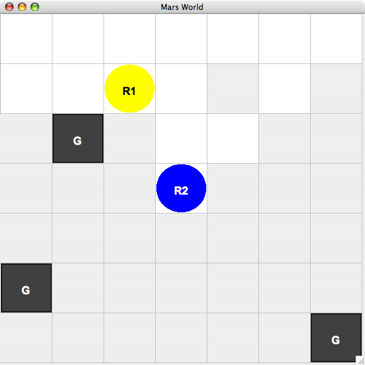
\includegraphics{figures/JasonEx-CR-ss1.png}
\end{quote}

\begin{enumerate}
\item All \Jason projects have a configuration file that ends with
  \texttt{.mas2j}, so to open the cleaning robots example, open the
  file \texttt{examples/cleaning-robots/mars.mas2j} that you'll find
  in the folder where you installed \Jason.

  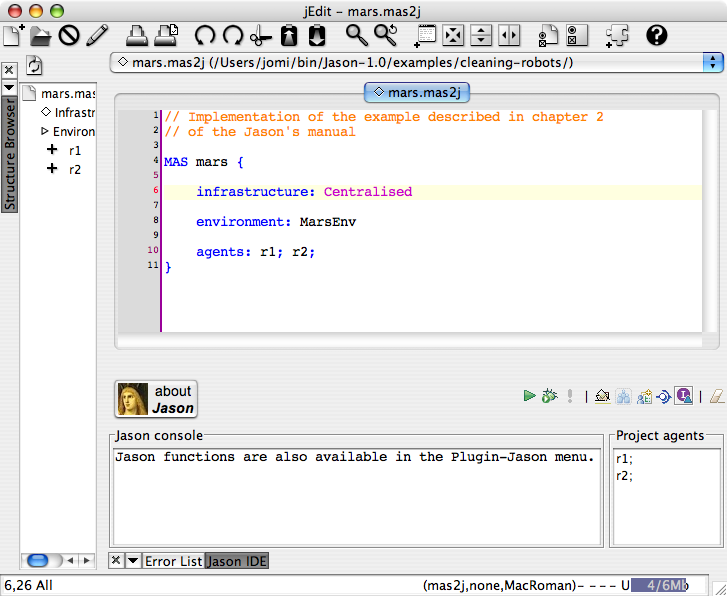
\includegraphics{figures/screen-mars.png}

  The project file defines the underlying infrastructure that has been
  chosen for that project (Centralised, Jade, Saci, ...), the Java
  class that implements the environment (MarsEnv), and the agents that
  belong to this application (r1 searches for pieces of garbage and
  r2 incinerates them).

\item To execute this application, click on the
  icon 
\includegraphics{figures/run.png}. Two windows are opened, the
  first is the application GUI and the second is the \Jason MAS
  Console where all print messages are shown (MAS is a common
  abbreviation of ``Multi-Agent Systems'').

  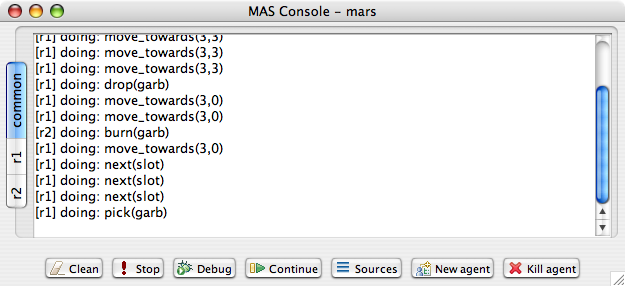
\includegraphics{figures/screen-masconsole.png}

\item To stop the MAS execution, click
  on 
\includegraphics{figures/suspend.png}, either in the MAS Console
  or in jEdit.

\end{enumerate}

\section{Creation of a simple example}

In this section we will create a new and simple example where two
agents, \texttt{bob} and \texttt{tom}, exchange greeting messages.

\begin{enumerate}

\item Click on the \includegraphics{figures/newProject.gif} icon and
  fill in the ``project name'' field with \emph{greeting}.

  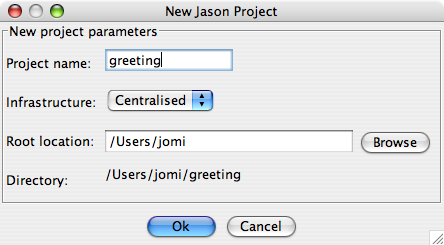
\includegraphics{figures/screen-newproject.png}

  (Don't worry about the syntax error in the project, it is caused
  because there are no agents in the system.)

\item Add a new agent called \texttt{bob} by clicking
  on \includegraphics{figures/newAgent.gif} and filling in only the
  ``agent name'' field. Note that the agent name has to be an
  AgentSpeak term, so it cannot start with an uppercase letter.

  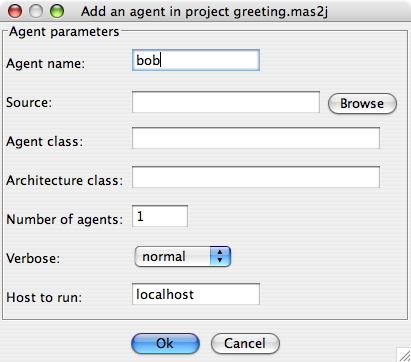
\includegraphics{figures/screen-newagent.png}

\item Do the same for \texttt{tom}.

\item As you can see, there is a skeleton for the agent's code: the
  agent has no beliefs, but an initial goal \texttt{start} and one
  plan to achieve this goal. The plan simply prints something when
  triggered.

  We will now change \texttt{tom}'s code so that it sends a ``hello''
  message to \texttt{bob}. To send messages, an \emph{internal action}
  called \texttt{.send} is used:

\begin{verbatim}
// Agent tom in project greeting.mas2j

!start.

+!start : true <- .send(bob,tell,hello).
\end{verbatim}

  In \texttt{bob}' code, we remove the \texttt{start} goal (and its
  related plan), leaving its program empty:
\begin{verbatim}
// Agent bob in project greeting.mas2j
\end{verbatim}


\item You can now run the project.  There is no output! However, in
  the MAS Console, click on the debug
  button \includegraphics{figures/debug.gif} and then select, in a new
  windows named ``Jason Mind Inspector'', the agent bob (if the
  agent's list is empty, click once in the run button). The mind
  inspector for \texttt{bob} will look as follows:

  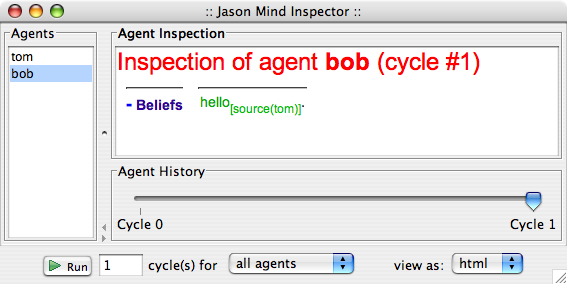
\includegraphics{figures/screen-mindinsp.png}

  Note the \texttt{bob} has a belief \texttt{hello[source(tom)]},
  which means that it received \texttt{tom}'s message.

\item Suppose now that we want \texttt{bob} to react to this
  message. Since the received message implies a belief addition, an
  event like \texttt{+hello[source(tom)]} is produced and may trigger
  the execution of the following plan:
\begin{verbatim}
// Agent bob in project greeting.mas2j

+hello[source(A)] <- .print("I received a 'hello' from ",A).
\end{verbatim}
  In the plan, \texttt{A} is a variable that contains the name of the
  sender. In AgentSpeak, as in Prolog, identifiers that start with
  uppercase letters are variables.

  If you run the new version, the output will be:

   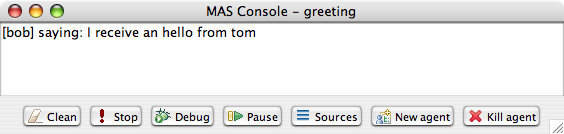
\includegraphics{figures/screen-hello.png}

\item Since \texttt{bob} is a polite agent, we will now make it send a
  hello back to \texttt{tom}:
\begin{verbatim}
// Agent bob in project greeting.mas2j

+hello[source(A)] 
  <- .print("I received a 'hello' from ",A);
     .send(A,tell,hello).
\end{verbatim}
  and \texttt{tom} does the same:
\begin{verbatim}
// Agent tom in project greeting.mas2j

!start.

+!start : true <- .send(bob,tell,hello).

+hello[source(A)] 
  <- .print("I receive an hello from ",A);
     .send(A,tell,hello).
\end{verbatim}

  Before running the system, think what you would expect to happen.
  Perhaps the agents will enter a kind of greeting loop?

\item Run the system and you will realise that there is no loop!  The
  reason is because when bob receives the second hello, it already has
  this belief in its belief base (BB). Since nothing changed in the
  BB, no event was produced, and thus no plan triggered.

\item If you want to use JADE as the infrastructure, change the
  project as follows:
\begin{verbatim}
MAS greeting {
    infrastructure: Jade

    agents:
        bob;
        tom;
}
\end{verbatim}
  Also change the configuration of the Jason Plugin to start the JADE
  Sniffer agent as well:

  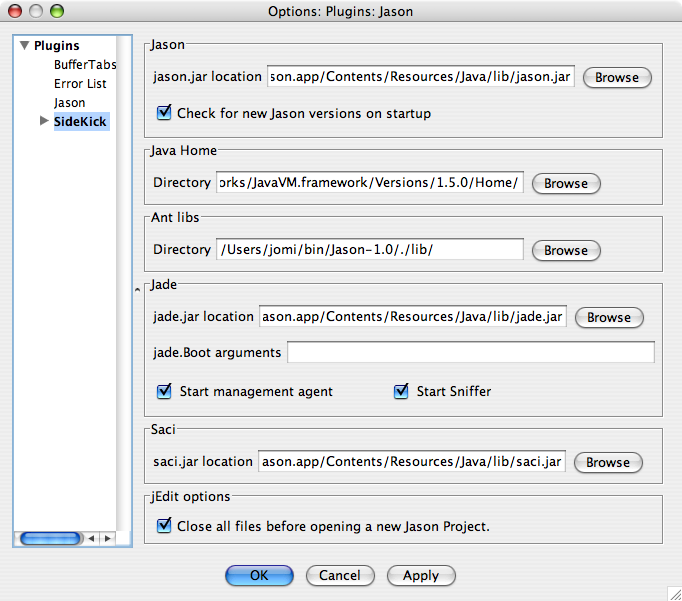
\includegraphics{figures/screen-confjade.png}

  The windows created when you run the system are shown below:

  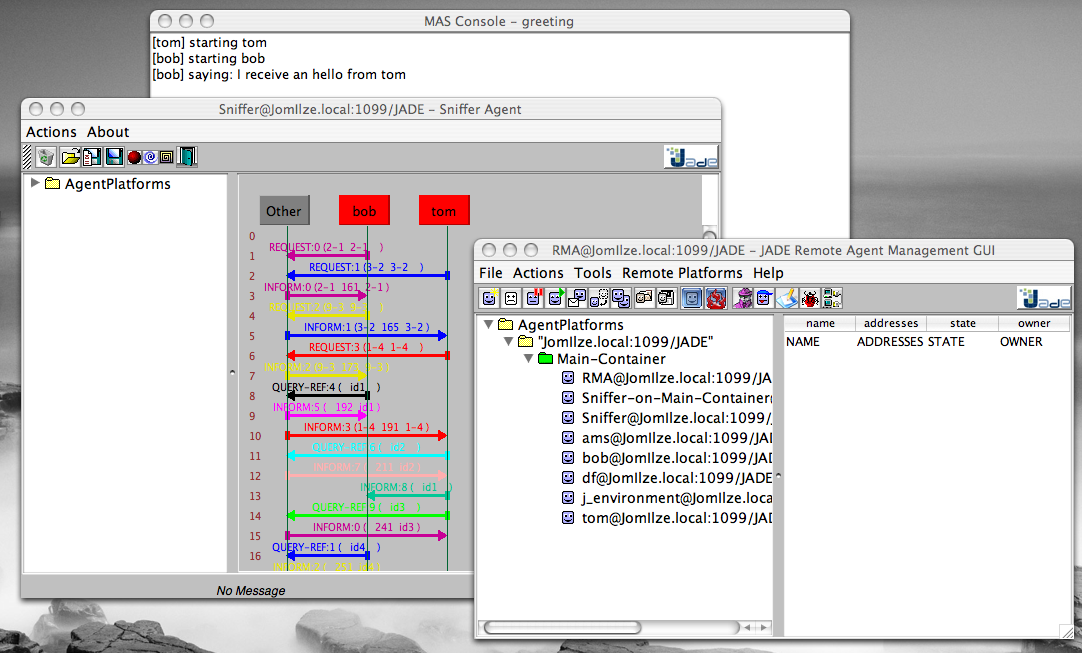
\includegraphics{figures/screen-runjade.png}

\end{enumerate}



\section{An example with environment}

In this section we will create a system where one agent will perform
one action in a simulated environment.

\begin{enumerate}
\item Create a new project called \texttt{testenv}.
\item Add one agent called \texttt{liz} with the following code:
\begin{verbatim}
// Agent liz in project testeenv.mas2j

!start.

+!start : true <- burn.
\end{verbatim}

  The plan's body has only the action, \texttt{burn}. Action here is
  meant to an \emph{environment action} (i.e., something that changes
  the state of the environment), and not internal actions (the ones
  which starts with a dot, or have a dot anywhere in their name).

\item The implementation of the \texttt{burn} action is done in an environment
  class. To create this class, click on the
  \includegraphics{figures/createEnv} icon and fill in the ``environment name''
  field with ``TestEnv''.  

  A skeleton for this class is added by \Jason. Change it to be
  exactly as follows:
\begin{verbatim}
// Environment code for project testenv.mas2j

import jason.asSyntax.*;
import jason.environment.*;
import java.util.logging.*;

public class TestEnv extends jason.environment.Environment {

  private Logger logger = Logger.getLogger("testenv.mas2j."+TestEnv.class.getName());

  /** Called before the MAS execution with the args informed in .mas2j */
  @Override
  public void init(String[] args) {    }

  @Override
  public boolean executeAction(String agName, Structure action) {
    if (action.getFunctor().equals("burn")) {
      addPercept(Literal.parseLiteral("fire"));
      return true;
    } else {
      logger.info("executing: "+action+", but not implemented!");
      return false;
    }
  }

  /** Called before the end of MAS execution */
  @Override
  public void stop() {
    super.stop();
  }
}
\end{verbatim}

  When an agent attempts to execute an environment action, the method
  \texttt{executeAction} of this class is executed. In this
  implementation, if the action \texttt{burn} is executed, a new
  percept \texttt{fire} becomes available to all agents.

\item Agent \texttt{liz} can now react to the perception of fire:
\begin{verbatim}
// Agent liz in project testeenv.mas2j

!start.

+!start : true <- burn.

+fire <- run.
\end{verbatim}

  (The implementation of the run action is left as an exercise.)
\end{enumerate}

\section{Exercise}

Imagine a very simple environment formed by 4 locations (identified by 1, 2, 3,
and 4) as in the figure below:

\begin{center}

\includegraphics{figures/ambiente.png}  
\end{center}

A vacuum-cleaner robot should be programmed in AgentSpeak to maintain
the environment clean. The available actions for the robot are:
\begin{itemize}
\item \texttt{suck}: remove dirt at the robot's position;
\item \texttt{left}: move the left;
\item \texttt{right}: move to right;
\item \texttt{up}: move up;
\item \texttt{down}: move down.
\end{itemize}
To help the robot decide what action to take, the following percepts
are given:
\begin{itemize}
\item \texttt{dirty}: the robot is in a dirty location; 
\item \texttt{clean}: the robot is in a clean location; 
\item \texttt{pos(X)}: the location of the robot is $X$ (0 < X < 5).
\end{itemize}

The following diagram, using the Prometheus notation, illustrates the
interactions between the robot and the environment.
\begin{center}
  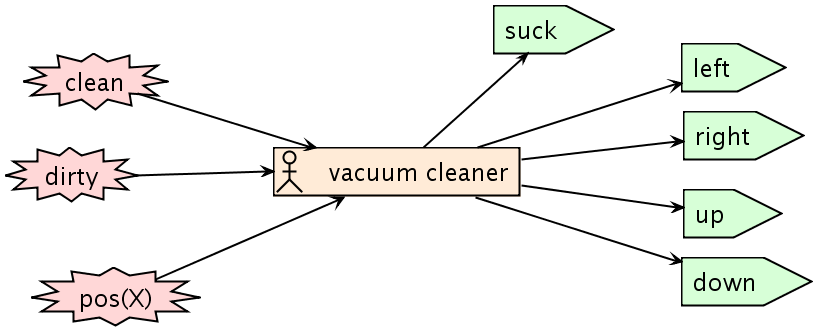
\includegraphics{figures/overview.png}
\end{center}

An implementation of the environment class is available
\htlink{here}{VacuumCleaning-1.zip}.


\textbf{Some tips}

You can start programming your agent by thinking about how it should
react to the available perception. For instance, what it should do
when it perceives "dirty"? The action "suck", of course! In AgentSpeak,
we program this reaction by means of a plan as follows:

\begin{verbatim}
+dirty <- suck. // when dirty is perceived, do the action suck
\end{verbatim}

So, an initial and very reactive agent can simply react to every
perception and be programmed as shown below (replace "someaction" for
the action you think is the most suitable, you might also want to
remove some of the plans):

\begin{verbatim}
+dirty  <- someaction.
+clean  <- someaction.
+pos(1) <- someaction.
+pos(2) <- someaction.
+pos(3) <- someaction.
+pos(4) <- someaction.
\end{verbatim}

Since all perception is also included in the belief base, they can
also be used to select the right plan, as in the following example:

\begin{verbatim}
+pos(1) : clean <- someaction.   // whenever I perceive I'm in pos(1) and
                                 // I believe that my position is clean, 
                                 // do some action.
\end{verbatim}


You will soon realise that this reactive approach has some limitation
in defining a good behaviour for our vacuum clearer. In fact, this agent
should be defined has having \emph{goals}, in particular, a persistent
goal of maintaining the house clean. The easiest way to define a
persistent goal is by a recursive plan; for example, the code below
implements the persistent goal (represented by p) of printing out "a":

\begin{verbatim}
!p.                   // initial goal
+!p <- .print(a); !p. // to achieve the goal p, print "a" 
                      // and after has p as a new goal.
\end{verbatim}


This document has shown a very limited range of \Jason's features; the
next section contains references where you can find further
information.

\section{More information}

You can find more information about \Jason at:
\begin{itemize}
\item \Jason website: \url{http://jason.sf.net} (mailing lists,
  publications, etc.)
\item \Jason book: \url{http://jason.sf.net/jBook}
\item The documentation included in the \texttt{doc} directory of the
  distribution (manual, FAQ, API, etc.)
\end{itemize}

\end{document}

